\documentclass[a0paper,fleqn]{betterposter}
\usepackage{graphicx}
\usepackage[colorlinks=true]{hyperref}

\begin{document}	
\betterposter{
%%%%%%%% MAIN COLUMN

\maincolumn{
%%%% Main space

	\textbf{Are there geographical biases in the study of language variation and change?}


}{
%%%% Bottom space

	\compactqrcode{frame-2.png}{Scan to access materials for this study on Github.}
}

}{
%%%%%%%% LEFT COLUMN

\title{Minority \\ Report}
\author{Caitlin Halfacre}
\author{Liam Keeble}

\institution{Newcastle University}

\section{Introduction}

Bias in science is unavoidable, and sociolinguistics is no different. In order to combat sources of bias, we must first identify its existence. With this study we aim to assess:
\begin{itemize}
\item whether there is bias towards studying some varieties of English over others.
\item whether location in relation to a research institution affect frequency of study of a variety of English.
\item other possible geographical/research characteristics (e.g. the existence of corpora/average income of the area) that may affects the frequency of studies published.
\end{itemize}

\section{Methods}

In order to meet our aims we:
\begin{itemize}
	\item Systematically searched \href{https://app.webofknowledge.com}{Web of Science} for studies on each particular variety of native English as identified by \href{https://en.m.wikipedia.org/wiki/List_of_dialects_of_English}{Wikipedia}.
	\begin{itemize}
		\item Search Term: (WC=(Linguistics)  AND  ((ALL="name of variety")  AND  ((ALL=sociolinguist*)  OR  (ALL=varia*)  OR  (ALL=change))))
		\item Document Type: All
		\item Timespan: 1982-2019 
	\end{itemize}
\end{itemize}
}
{
%%%%%%%%%Right column
	\section{Methods cont.}	
\begin{itemize}
%	\item Wikipedia was used as it serves as a kind of public self-identifier for speakers of speaking different varieties.
	\item pre-screened the resulting list and removed based on the inclusion criteria:
	\begin{itemize}
		\item the study assesses language variation or change
		\item study assesses the variety of English specified in the search
	\end{itemize}
	\item The remaining studies from each search were counted.

	\item Regional average uk disposable incomes were obtained from the office for national statistics.
	\item The existence of corpora for a variety was obtained by google searches.
	\item Geographical distance between a variety and the nearest linguistics dept. were obtained using the ggmaps package in R.
	
	\item The metropolitan status of varieties was determined by whether or not the variety names corresponded to a English city.
\end{itemize}



\section{Results}


	\begin{itemize}
	\item The figure presented below shows the relationships between each predictor in a poisson regression and number of studies found for different varieties of English. 
	\end{itemize}
	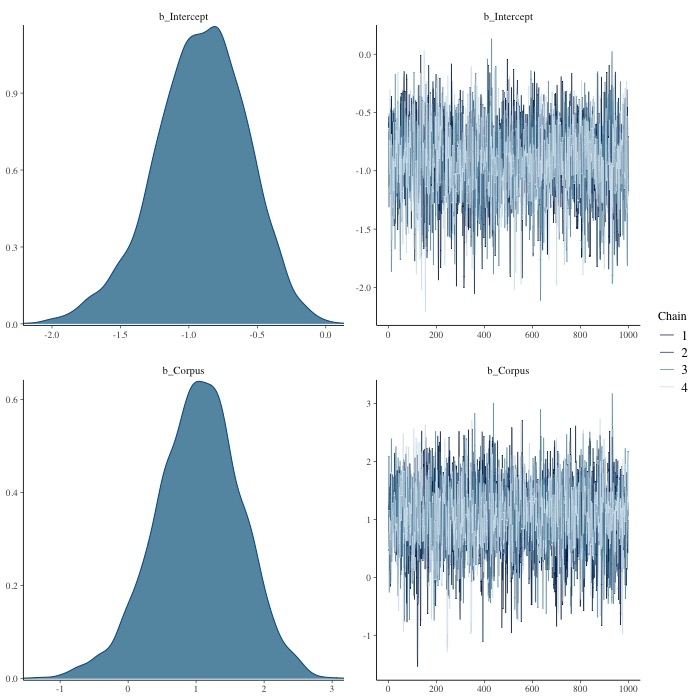
\includegraphics[scale=1.1]{new.jpg}
	

}


\end{document}



